\documentclass[11pt,a4paper,twoside]{book}

%include the configuration file for layout
%Have a look in this file it has some useful commands defined
\usepackage{setspace}
\usepackage{geometry}
\usepackage[toc,page]{appendix}
\usepackage{lipsum}
\usepackage[export]{adjustbox}
\usepackage[T1]{fontenc}
\usepackage{textcomp}
\usepackage{epsfig,graphics}
\usepackage[font=small,justification=centering]{caption}
\usepackage{graphicx}
\usepackage{titlesec}
\usepackage[style=numeric,sorting=none]{biblatex}
\usepackage{siunitx}
\usepackage{wrapfig}
\usepackage{subcaption}
\usepackage{color}
\usepackage{multirow}
\usepackage{hyperref}


%%%%%%%%%%%%%%%%%%%%%%%%%%%%%%%%%%%%%%%%%%%%%%%%%%%%%%%%%%%%%%%%%%%%%%%%%%%%%%
% Details of your dissertation
%%%%%%%%%%%%%%%%%%%%%%%%%%%%%%%%%%%%%%%%%%%%%%%%%%%%%%%%%%%%%%%%%%%%%%%%%%%%%%
\newcommand{\projectTitle}{Surface Normal Estimation from RGB Images}
\newcommand{\fullname}{Mohammad Kaykanloo}
\newcommand{\degreeTitle}{MSc Advanced Computer Science (Intelligent Systems)}
\newcommand{\session}{2016/2017}

%%%%%%%%%%%%%%%%%%%%%%%%%%%%%%%%%%%%%%%%%%%%%%%%%%%%%%%%%%%%%%%%%%%%%%%%%%%%%%
% Change the geometry of the page to have a 25 mm binding edge
%%%%%%%%%%%%%%%%%%%%%%%%%%%%%%%%%%%%%%%%%%%%%%%%%%%%%%%%%%%%%%%%%%%%%%%%%%%%%%
 \geometry{
 a4paper,
 left=25mm,
 right=25mm,
 top=25mm,
 bottom=20mm,
 heightrounded,
 }
 
%%%%%%%%%%%%%%%%%%%%%%%%%%%%%%%%%%%%%%%%%%%%%%%%%%%%%%%%%%%%%%%%%%%%%%%%%%%%%%
% Commands to set the line spacing
%%%%%%%%%%%%%%%%%%%%%%%%%%%%%%%%%%%%%%%%%%%%%%%%%%%%%%%%%%%%%%%%%%%%%%%%%%%%%%
 %\singlespacing
 \onehalfspacing
 %\doublespacing
 
%%%%%%%%%%%%%%%%%%%%%%%%%%%%%%%%%%%%%%%%%%%%%%%%%%%%%%%%%%%%%%%%%%%%%%%%%%%%%%
% Spacing for the chapter header
%%%%%%%%%%%%%%%%%%%%%%%%%%%%%%%%%%%%%%%%%%%%%%%%%%%%%%%%%%%%%%%%%%%%%%%%%%%%%%
 \titleformat{\chapter}[display]
    {\normalfont\Huge\bfseries}{\vspace*{-1\baselineskip}\chaptertitlename\ \thechapter}{15pt}{\huge}
\titlespacing*{\chapter}{0pt}{0pt}{15pt}

\renewcommand\bibname{References}

%%%%%%%%%%%%%%%%%%%%%%%%%%%%%%%%%%%%%%%%%%%%%%%%%%%%%%%%%%%%%%%%%%%%%%%%%%%%%%
% Some shortcuts that maybe useful
%%%%%%%%%%%%%%%%%%%%%%%%%%%%%%%%%%%%%%%%%%%%%%%%%%%%%%%%%%%%%%%%%%%%%%%%%%%%%%
\DeclareTextCommandDefault{\textcopyright}{\textcircled{c}}
 
%%%%%%%%%%%%%%%%%%%%%%%%%%%%%%%%%%%%%%%%%%%%%%%%%%%%%%%%%%%%%%%%%%%%%%%%%%%%%%
% Bibliography
%%%%%%%%%%%%%%%%%%%%%%%%%%%%%%%%%%%%%%%%%%%%%%%%%%%%%%%%%%%%%%%%%%%%%%%%%%%%%%
\DefineBibliographyStrings{english}{%
  bibliography = {References},
  references = {References},
}
\addbibresource{refs.bib}

%%%%%%%%%%%%%%%%%%%%%%%%%%%%%%%%%%%%%%%%%%%%%%%%%%%%%%%%%%%%%%%%%%%%%%%%%%%%%%
% Images default path
%%%%%%%%%%%%%%%%%%%%%%%%%%%%%%%%%%%%%%%%%%%%%%%%%%%%%%%%%%%%%%%%%%%%%%%%%%%%%%
\graphicspath{ {Images/} }

%%%%%%%%%%%%%%%%%%%%%%%%%%%%%%%%%%%%%%%%%%%%%%%%%%%%%%%%%%%%%%%%%%%%%%%%%%%%%%
% Layout for the front cover !!!!! YOU SHOULD NOT HAVE TO CHANGE THIS!!!!!
%%%%%%%%%%%%%%%%%%%%%%%%%%%%%%%%%%%%%%%%%%%%%%%%%%%%%%%%%%%%%%%%%%%%%%%%%%%%%%
 
\newcommand{\frontcover}{
% The title page:
\begin{titlepage}
\newgeometry{left=25mm,right=25mm,top=45mm,bottom=0.1cm}

\begin{minipage}[t]{7cm}
\noindent\textbf{\Large{School of Computing}}\\
{\fontfamily{ptm}\selectfont 
\uppercase{faculty of engineering}
}
\end{minipage}
\hfill
\begin{minipage}[t]{7cm}
\vspace*{-25pt}

\includegraphics[scale=0.2,right]{logo_black.png}
\vspace*{-1pt}
\end{minipage}

\noindent\makebox[\linewidth]{\rule{\paperwidth}{0.4pt}}

\centering
\vspace*{37mm}
\textbf{\Large\projectTitle}\\
\vspace*{10mm}
\textbf{\large\fullname}\\
\vspace*{10mm}
\textbf{Submitted in accordance with the requirements for the degree of}\\
\textbf{\degreeTitle}\\
\vspace*{10mm}
\session\\
\restoregeometry
\end{titlepage}
}

%%%%%%%%%%%%%%%%%%%%%%%%%%%%%%%%%%%%%%%%%%%%%%%%%%%%%%%%%%%%%%%%%%%%%%%%%%%%%%
% Define a new environment for the dissertation summary
%%%%%%%%%%%%%%%%%%%%%%%%%%%%%%%%%%%%%%%%%%%%%%%%%%%%%%%%%%%%%%%%%%%%%%%%%%%%%%
\newenvironment{dissertationsummary}
 	{\cleardoublepage \null 
 		\begin{center}%
			\textbf{Summary}
		\end{center}}%
	{\vfill \null }
	
%%%%%%%%%%%%%%%%%%%%%%%%%%%%%%%%%%%%%%%%%%%%%%%%%%%%%%%%%%%%%%%%%%%%%%%%%%%%%%
% License line of captions
%%%%%%%%%%%%%%%%%%%%%%%%%%%%%%%%%%%%%%%%%%%%%%%%%%%%%%%%%%%%%%%%%%%%%%%%%%%%%%
\newcommand{\caplicense}[1]{\\ \scriptsize \textit{#1}}

\begin{document}
%The prelude is everything upto the start of chapter 1
\pagenumbering{roman}
\frontcover

\clearpage
\noindent The candidate confirms that the following have been submitted.\\

\begin{table}[ht!]
\begin{tabular}{|p{0.3\textwidth}|p{0.3\textwidth}|p{0.3\textwidth}|}
\hline 
Items & Format & Recipient(s) and Date \\ 
\hline 
Project Report & Report & SSO (DD/MM/YY) \\ 
\hline 
Dataset & URL & Supervisor, Assessor (DD/MM/YY) \\ 
\hline 
Implementation & Software codes and URL & Supervisor, Assessor (DD/MM/YY) \\ 
\hline 
\end{tabular} 
\end{table}

\noindent Type of project: Exploratory Software
\vspace{\fill}\\
\noindent The candidate confirms that the work submitted is their own and the appropriate credit has been given where reference has been made to the work of others.
\vspace{\fill}\\
\noindent I understand that failure to attribute material which is obtained from another source may be considered as plagiarism.
\vspace{\fill}\\
\flushright(Signature of Student) \rule{50mm}{1pt}
\flushleft
\vspace{\fill}
\textcopyright~\session~The University of Leeds and~\fullname
% Summary

\begin{dissertationsummary}
This project explored a deep learning approach for the task of pixel-wise surface normal estimation from monocular RGB images. At first, an analysis of the previous research was conducted. Then, data required for use in this project was obtained from two publicly available data sets. Software code was developed to compute the ground truth surface normal maps based on two different methods and the results were used to produce the final data sets.

A deep learning pipeline was developed and a baseline network architecture was implemented. Based on the insights gained from the literature review and analysis of the state of the art methods, different modifications to the baseline model were investigated. In particular, improvements over baseline results were explored in respect to two aspects: network architectures, and the quality of the data set.

Finally, well-established evaluation metrics were implemented and the quantitative and qualitative result of evaluation were presented and compared to the state of the art methods.  

\end{dissertationsummary}

\clearpage
\centering\textbf{Acknowledgements}
\flushleft
<The page should contain any acknowledgements to those who have assisted with your work. Where you have worked as part of a team, you should, where appropriate, reference to any contribution made by other to the project.>

Note that it is not acceptable to solicit assistance on `proof reading' which is defined as the ``the systematic checking and identification of errors in spelling, punctuation, grammar and sentence construction, formatting and layout in the test'';\\ see http://www.leeds.ac.uk/gat/documents/policy/Proof-reading-policy.pdf.



% The contents
\tableofcontents

% The list of figures and tables Uncomments the 3 following lines
%to see a list of tables and list of figures.
%\clearpage
%\listoffigures
%\listoftables


% Change to arabic numerals
\pagenumbering{arabic}

%include as many chapters as you have.
%the chapters are in a directory called Chapters
\chapter{Introduction}
\label{Introduction}

\section{Context}

Arguably, humans rely on their sense of sight more than any other sense in understanding the world around them. Finding our way in a busy street, locating a book on a shelf in a library and interacting with hundreds of objects in our everyday life are some of examples that require extensive use of visual cues. We can not only recognise objects and locations, but also create a 3D structure of the scene in our mind. Even by looking at a single image, we can answer complex questions about position, orientation, and relation of objects. 

As technologies such as augmented reality, self-driving cars, drones, and robotics in general, progress towards finding more use cases in our every day lives, the need for better scene understanding in real 3D space increases. By advent of intelligent personal assistant softwares and smarter applications, providing more useful features and better user experience depends on understanding the real world that users live in it.

Scene understanding is one of the most fundamental problems in computer vision. It is very challenging to solve this problem by only using 2D visual data captured by ordinary cameras. Thus, hardware manufacturers have tried to make this task easier by providing more information about the 3D space; using a variety of camera arrays, structured light 3D scanners, and time-of-flight (ToF) sensors. 3D vision systems use these sensors to measure, map, locate, and reconstruct the three dimensional structure of the environment for visual perception tasks.  

Data provided by these sensors, plays a crucial role in many currently popular products in fields of augmented reality, robotics, biometric facial recognition, and gesture detection (e.g. Microsoft Kinect, Apple FaceID, and Tesla Autopilot). But in many applications, access to these sensors is not simply possible. For example, the vast amount of images and videos currently available on the internet, provide no extra 3D information about their content. On the other hands, in comparison to humans, software systems are unable to fully exploit the visual information that 2D images contain. Therefore, there is still a strong need for developing more advanced scene understanding and reconstruction systems that are based on 2D input data.      

Estimating the orientation of surfaces in an image, is an important step in reconstructing a 3D model of the scene. Recently, the surface normal estimation from monocular RGB images, has been an active area of research in computer vision. Tackling this problem is the main topic of this M.Sc. project. 

\pagebreak

\section{Problem Statement} \label{problemstatement}

Before any further discussion, a precise definition of the problem is needed. In this project, the problem of pixel-wise surface normal estimation from monocular RGB images of the indoor scenes is addressed. 

The RGB images are captured from indoor environments with realistic scene layout such as bedrooms, living rooms, kitchens, and offices. Figure \ref{fig:scene} illustrates a typical scene layout and viewpoint. 

\begin{figure}[h]
    \centering
    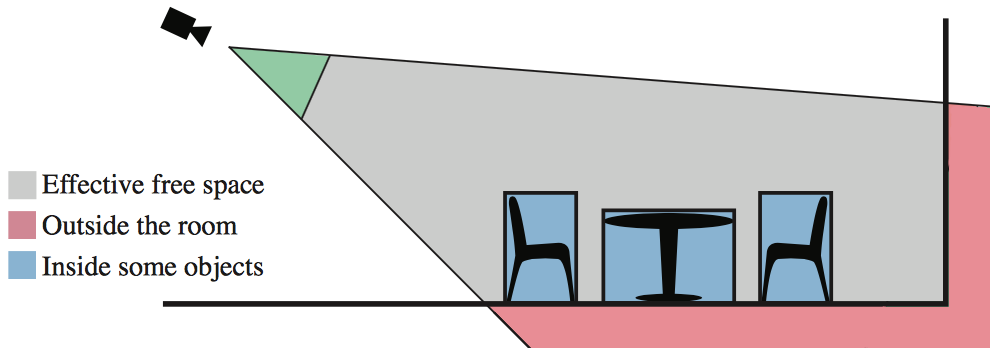
\includegraphics[scale=0.35]{Scene}
    \caption{Schematic view of a scene, adapted from \cite[p.~5]{sun}}
    \label{fig:scene}
\end{figure}

Given an RGB image as input, the estimated surface normal map is expected as output. Samples of RGB images and the corresponding normal maps are illustrated in figure \ref{fig:gt}. 

\begin{figure}[h]
    \centering
    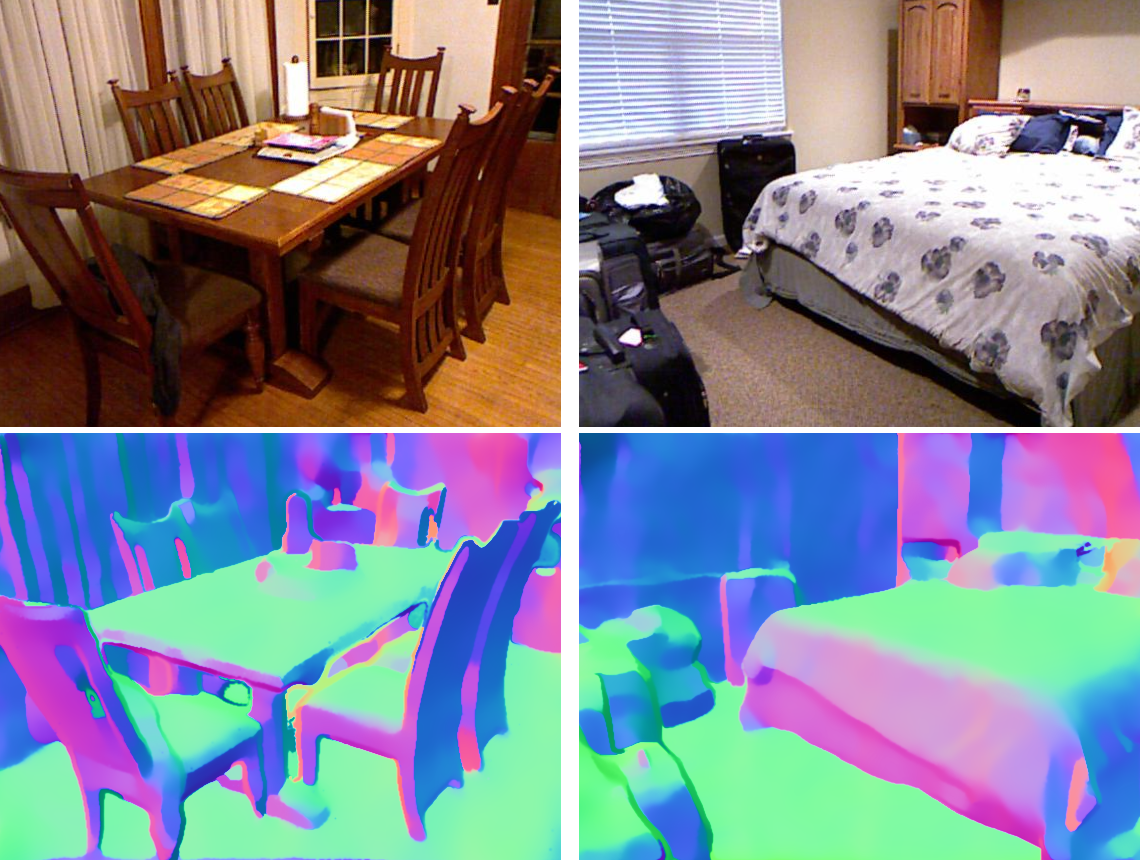
\includegraphics[scale=0.3]{GT}
    \caption{Top: RGB images of indoor scenes, Bottom: corresponding surface normal maps \\
    Normal legend: {\color{blue} $blue\rightarrow X (horizontal)$}; {\color{green} $green\rightarrow Y (vertical)$}; {\color{red} $red\rightarrow Z (perpendicular\ to\ image)$}.}
    \label{fig:gt}
\end{figure}


\section{Proposed Solution}

In last few years, deep learning has made major breakthroughs in field of computer vision.  Deep neural networks (DNNs) have achieved impressive performance in challenging tasks such as image classification, semantic segmentation, and image compression. DNNs have started to even exceed human performance in tasks such as image classification \cite{humanvsdnn}. Therefore it is not surprising that current state of the art solutions for the task of surface normal estimation are all based on deep learning. 

Based on the promising achievements of deep neural networks, and the huge gap between the results yielded by using these networks in comparison to traditional methods in similar problems, a solution based on DNNs was chosen as the preferred approach for this project. At first, a baseline network architecture was implemented and after training the model, the estimated surface normal maps were evaluated.  Afterwards, based on the insights gained from the literature review and analysis of the state of the art methods, different modifications to the baseline model were investigated. In particular, improvements over baseline results were explored in respect to two aspects: network architectures, and the quality of data set.   

\section{Project Aim}

This project explored a deep learning approach for the task of surface normal estimation. The data needed for training and evaluation of the system, was acquired by using publicly available data sets. Different network architectures were implemented and finally, well-established evaluation metrics were used to compare the results with the previous research in this field. 

\subsection{Objectives}

\begin{itemize}
    \item Data set and ground truth acquisition
    \item Analysing the state-of-the-art methods
    \item Proposing a new method or improvements over current methods and
implementing it
    \item Evaluating the method and comparing with other methods
\end{itemize}

\subsection{Deliverables}

\begin{itemize}
    \item Data set
    \item Analysis of the state-of-the-art methods
    \item Source code and algorithms
    \item Evaluation results
\end{itemize}

\section{Planning and Project Management}

Before starting the work on this project, a period of two months was spent on background study and literature review. During this period, works relevant to the subject of this project were identified, and the theoretical aspects of the solutions discussed in existing research, were studied. A better understanding of the problem, and a proposed solution were the outcomes of this process. 

\subsection{Initial Plan}
To guide the project execution, an initial plan was devised and the project was broken down to four main tasks: 

\begin{itemize}
    \item \emph{Data Acquisition and Preparation}: preparing the data sets required for training and evaluation of the system
    \item \emph{Analysis of Related Work}: studying the source codes released by relevant works and reproducing their results
    \item \emph{Implementation and Evaluation}: implementing the system and evaluating the results
    \item \emph{Report Writing}: writing the project report
\end{itemize}

Based on these tasks, an initial project schedule for a period of three months was created (figure \ref{fig:initialplan}). 

\begin{figure}
    \centering
    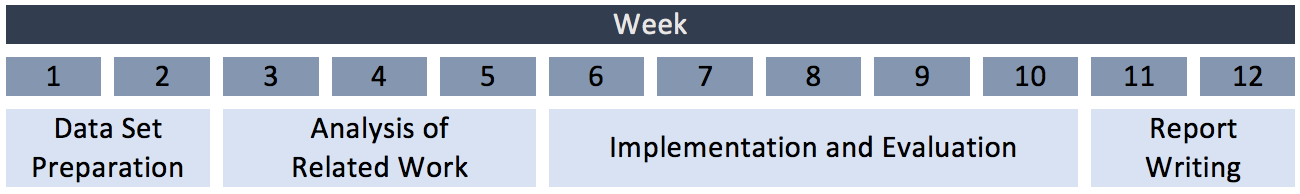
\includegraphics[width=\textwidth]{InitialPlan}
    \caption{Initial project plan}
    \label{fig:initialplan}
\end{figure}

\subsection{Revised Plan}
In reality, the time that was spent on different tasks was different with what initially was planned. Because of difficulties in data set preparation task, one more week than expected was spent on this task. Also, analysis of related work took one week less than expected. After two months, in a progress meeting with supervisor and assessor of the project, the project plan was reconsidered. 

\begin{figure}[h]
    \centering
    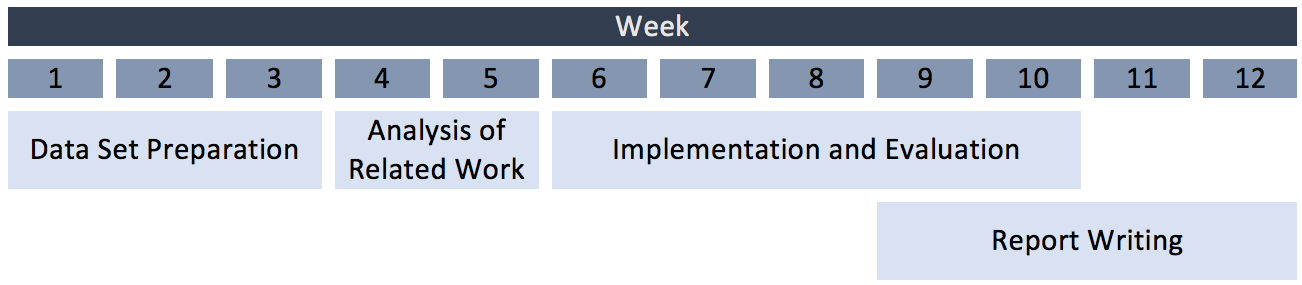
\includegraphics[width=\textwidth]{RevisedPlan}
    \caption{Revised project plan}
    \label{fig:revisedplan}
\end{figure}

Figure \ref{fig:revisedplan} illustrates the revised project plan. Based on the provided suggestions, the time considered for writing the project report was extended to four weeks, starting in parallel to last weeks of project implementation and evaluation. 

\subsection{Methodology}
The methodology used for this project was mainly based on performing a series of experiments to gradually design better network architectures. The implementation and evaluation task was conducted based on the workflow illustrated in figure \ref{fig:workflow}. After preparing the data sets, for each experiment, a sequence of activities was carried out: designing a network architecture, implementation, training the network, evaluation of the predicted outputs, analysis of the results and documentation. After each experiment, based on the outcome, a new experiment was designed to investigate a hypothesis or improve the network architecture. This process was repeated for the limited time that was available to this phase of project.  

\begin{figure}
    \centering
    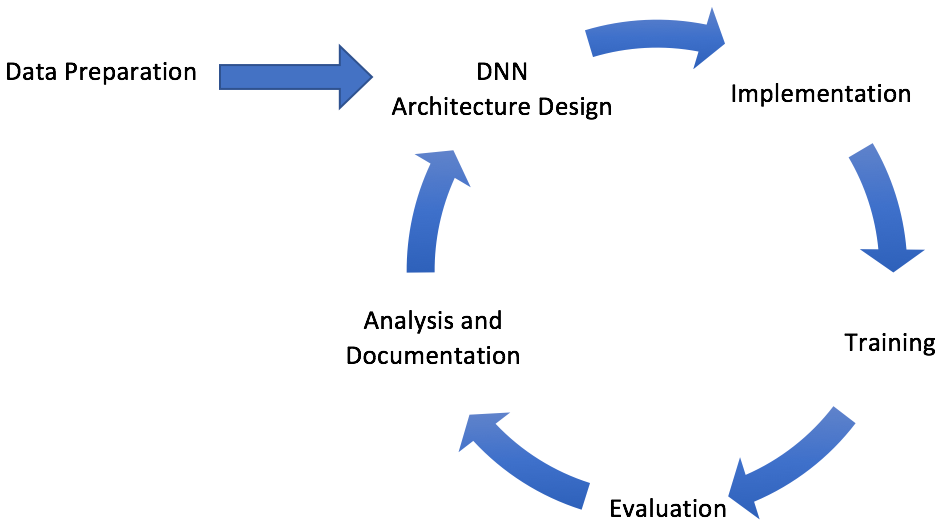
\includegraphics[scale=0.3]{Workflow}
    \caption{Project Workflow}
    \label{fig:workflow}
\end{figure}

\subsection{Risk Assessment}

After literature review, an assessment of the risks associated with this project was carried out. Consequently, difficulty in reproducing the results of the previous research, was identified as one of the main risks in this project. Therefore, it was decided that in case of facing such problem, instead of reproducing the results, the reported results would be used as a basis for comparing the outcome of this project with the state of the art.  

\chapter{Background}
\label{Background}

\section{Deep Learning}
\section{Transfer Learning}
\section{Related Work}


\chapter{Data Set}
\label{Dataset}

\section{Overview}

In success of any software system that is based on deep neural networks, two main factors play a crucial role: network architecture and training data set. Although, a good network design is necessary for getting acceptable results; without an appropriate data set, training the network and getting any result is not possible. In fact, not only the quality of data set matters, but also as \citeauthor*{data} \cite{data} show, the performance of deep neural networks in vision tasks increases logarithmically based on volume of training data. 

For the task of surface normal estimation from RGB images of indoor scenes, a data set containing the RGB images and the corresponding surface normal maps is needed. As mentioned in related work section (page \pageref{sec:relatedwork}), it is possible to indirectly calculate the needed surface normal maps by using the depth map of the images. Therefore, to acquire such data set, a collection of images and their corresponding depth maps should be obtained; either by directly taking various pictures of indoor scenes or by using publicly available RGB-Depth data sets. 

Capturing new images is not only time consuming, but also makes it difficult to compare the results of the experiments with previously published results. Therefore, in this project, a publicly available RGB-D data set (NYU Depth V.2 \cite{silberman}) is used. All related work discussed in section \ref{sec:relatedwork}, use this data set for training their models. Also, to explore the effect of using a higher quality data set on improving network performance, a more recently released data set (SUN RGB-D \cite{sun}) is used in this project. 

There are several methods for computing the surface normal maps based on the depth map of the scene. For consistency with past research in this field and producing comparable results, this project used surface normal maps computed by using two more popular methods of \citeauthor*{ladicky} \cite{ladicky} and \citeauthor*{silberman} \cite{silberman}. These methods and the aforementioned data sets are discussed in next sections. 

\section{Publicly Available RGB-D Data Sets }

There are many existing RGB-D data sets available; but, only a few of them are suitable for the purpose of this project. For example, some data sets (such as \cite{objectdataset} and \cite{bigbird}) use a turntable for capturing the image of objects, instead of using real-world scenes. Even in data sets that use real-world indoor scenes, some of them (such as Berkeley 3-D Object Dataset \cite{b3do}) contain unrealistic scene layouts (e.g. snapshot of a computer mouse on the floor) or have a small size. In the following sections, two of the data sets that are more suited for use in this project are briefly introduced.

\subsection{NYU Depth V.2}

This data set has been the most popular data set for the task of surface normal estimation of indoor scenes. It is comprised of 1,449 pairs of aligned RGB and depth images, gathered from a wide range of commercial and residential buildings in three different US cities. These images are extracted from short video sequences captured by Microsoft Kinect version 1, from 464 indoor scenes across 26 scene classes. 

The data set has three components: the raw data (rgb, depth and accelerometer) as provided by the Kinect, preprocessed RGB and depth images, and a toolbox for data manipulation. In preprocessed part of the data set, in addition to the projected depth maps, a set of preprocessed depth maps whose missing values have been filled in (using the colourisation scheme of \citeauthor*{colorization} \cite{colorization}) is also included. This data set also provides meta-data about each image; which is irrelevant to this project (such as dense per-pixel labeling for each image). Figure \ref{fig:nyu} illustrates a few samples of this data set. 

\begin{figure}
    \centering
    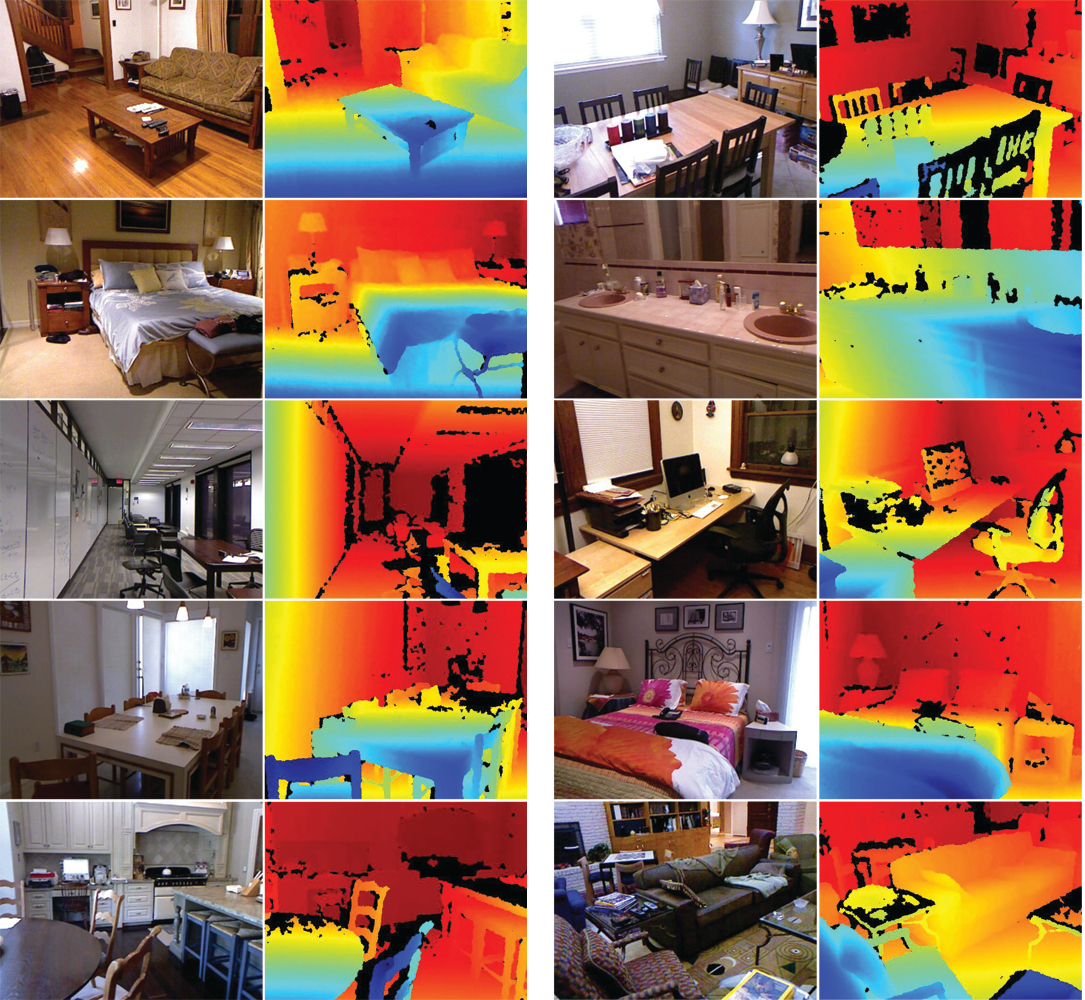
\includegraphics{NYU}
    \caption{NYU Depth V.2 data set, samples of the RGB images and the corresponding depth maps (missing data is coloured in black)\cite{silberman}}
    \label{fig:nyu}
\end{figure}

\citeauthor*{silberman} also suggest a train/test split for the samples of the data set. In this project, this split was used for selecting the samples for training and evaluation processes. The preprocessed samples and the toolbox are provided in format of MathWorks MATLAB files. 

\subsection{SUN RGB-D}

Princeton SUN RGB-D data set \cite{sun}, is a super-set of the NYU Depth V.2 \cite{silberman} data set. To construct this data set, \citeauthor*{sun} \cite{sun} capture 3,784 images using Microsoft Kinect v2 and 1,159 images using Intel RealSense sensors. They also include the 1,449 images from the NYU Depth V.2 data set and manually select 554 realistic scene images from the Berkeley B3DO Dataset \cite{b3do}. Finally, by including the manually selected 3,389 distinguished frames from the SUN3D \cite{sun3d} videos captured by Asus Xtion sensor, the total number of images in this data set reaches 10,335.

These RGB-D images are extracted from short videos captured from indoor scenes (such as universities, houses, and furniture stores) in North America and Asia. Like NYU Depth V.2, the raw depth maps captured by the depth sensors in this data set is not perfect; due to measurement noise, reflection of surfaces like mirrors, and occlusion boundaries. 

Also, the resolution of RGB images and the quality of raw depth maps captured by different sensors is not equal. Intel RealSense outputs noisier depth maps with more missing values, while Asus Xtion and Kinect v.1's depth maps have observable quantisation effects. Kinect v.2 captures depth maps with more details, but it is more sensitive to reflection and dark colours. Thus, to improve these depth maps, \citeauthor*{sun} propose an algorithm that uses depth data captured during multiple frames of the video, to obtain a single refined depth map for each image (Figure \ref{fig:sensors}). 

\begin{figure}
    \centering
    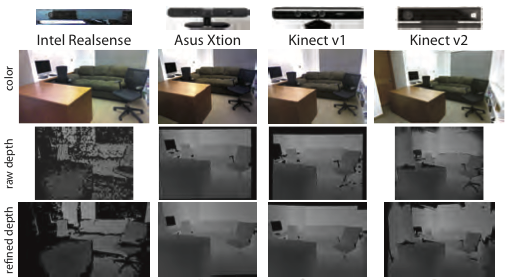
\includegraphics[width=\textwidth]{Sensors}
    \caption{Comparison of the four RGB-D sensors and the refinements in depth maps achieved by using the algorithm of \citeauthor*{sun} \cite[p.~2]{sun}}
    \label{fig:sensors}
\end{figure}

Alongside this data set, a toolbox (MathWorks MATLAB files) for loading and visualisation of data is also provided. The RGB images and depth maps are presented as PNG files.    

\section{Surface Normal Maps} \label{sec:surfnormmap}

As mentioned earlier, several different methods are used for computing the surface normal maps from depth data. In all related work discussed in chapter \ref{Background}, the published results are evaluated based on the surface normal maps computed by \citeauthor*{ladicky} \cite{ladicky} on the testing data set. For training the network, the raw data from the training data set is used. Because \citeauthor*{ladicky} have not published the surface normal maps for the raw data of the NYU Depth V.2 data set \cite{silberman}, the method of \citeauthor*{silberman} \cite{silberman} is used for computing these normal maps. \citeauthor*{dharmasiri} \cite{dharmasiri} also additionally evaluated their result based on the surface normal maps computed by the method of \citeauthor*{spek} \cite{spek}. 

\pagebreak

In this project, the method of \citeauthor*{silberman} \cite{silberman} was used for computing the surface normal maps in SUN RGB-D data set \cite{sun}. To get comparable results, surface normal maps provided by \citeauthor*{ladicky} \cite{ladicky} were used in evaluating the output of the networks.

In method used by \citeauthor*{silberman} \cite{silberman}, first by using the intrinsic parameters of the camera, the depth points are projected from image plane to the 3D world coordinates. Then, for the neighbouring sets of points in the 3D point cloud that their distance is not too large, a least-square plane is fitted. The normal vectors of these planes are the computed surface normals corresponding to the depth map points.  

On the other hand, \citeauthor*{ladicky} \cite{ladicky} first apply a denoising technique (based on the second order Total Generalized Variation (TGV) \cite{tgv}) on depth data. Then, normals are computed on the 3D point cloud for each point in a local 3D spatial neighbourhood. Finally, to estimate the point-wise normals, a least squares regression kernel in a RANSAC scheme is utilised in order to preserve surface edges \cite[p.~10]{ladicky}. 

The difference between these methods is due primarily to the fact that \citeauthor*{ladicky} \cite{ladicky} uses a more aggressive smoothing which results in flatter areas, while \citeauthor*{silberman} \cite{silberman} produces noisier results but with more details present \cite[p.~5]{eigen}. Figure \ref{fig:normalmethods} illustrates the difference in output of these methods.

\begin{figure}[h]
    \centering
    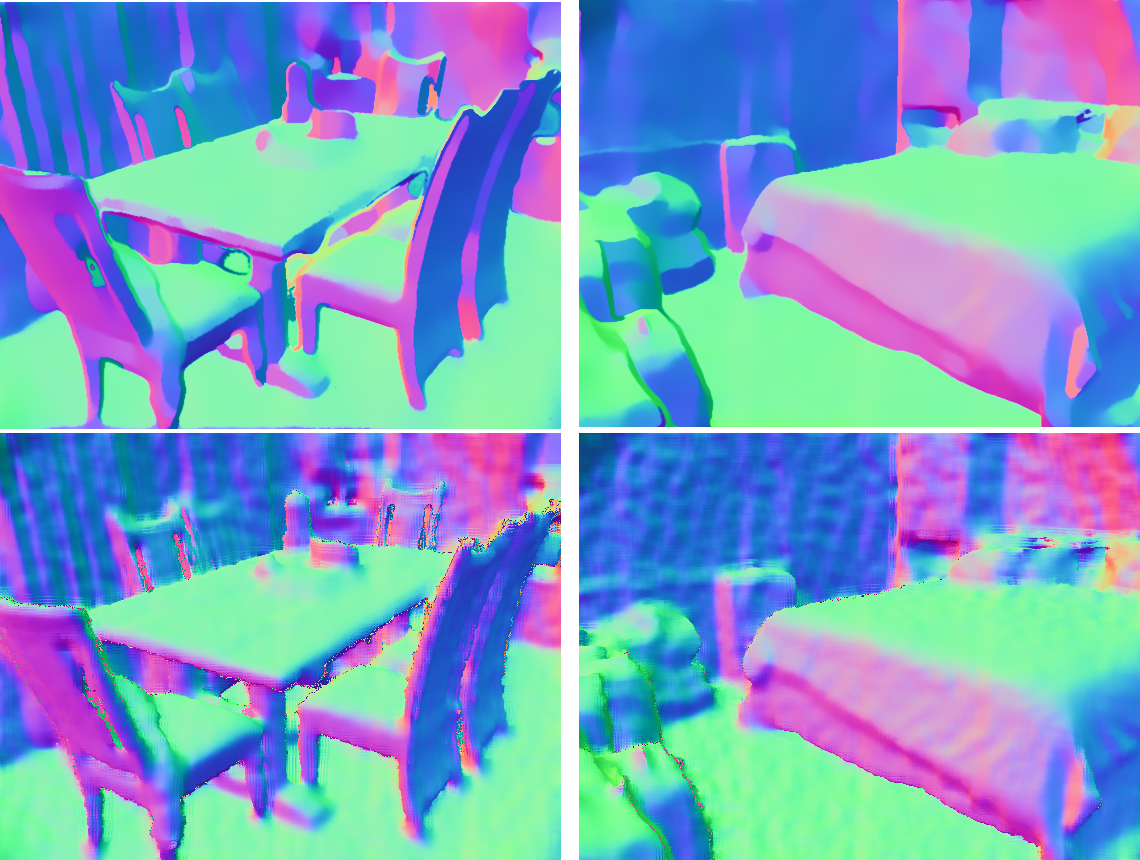
\includegraphics[width=\textwidth]{NormalMethods}
    \caption{Comparison of normal maps computed by different methods \\
    Top: based on \citeauthor*{ladicky} \cite{ladicky} , Bottom: based on \citeauthor*{silberman} \cite{silberman}  }
    \label{fig:normalmethods}
\end{figure}

\pagebreak

To reduce the noise presented in the output of \citeauthor*{silberman}'s method \cite{silberman}, inspired by the work of \citeauthor*{wang}, a denoising technique (total variation regularised least-squares deconvolution \cite{chan}) was applied on the computed normal maps in this project. Figure \ref{fig:denoisedsilberman} illustrates the results obtained by applying this method.

\begin{figure}
    \centering
    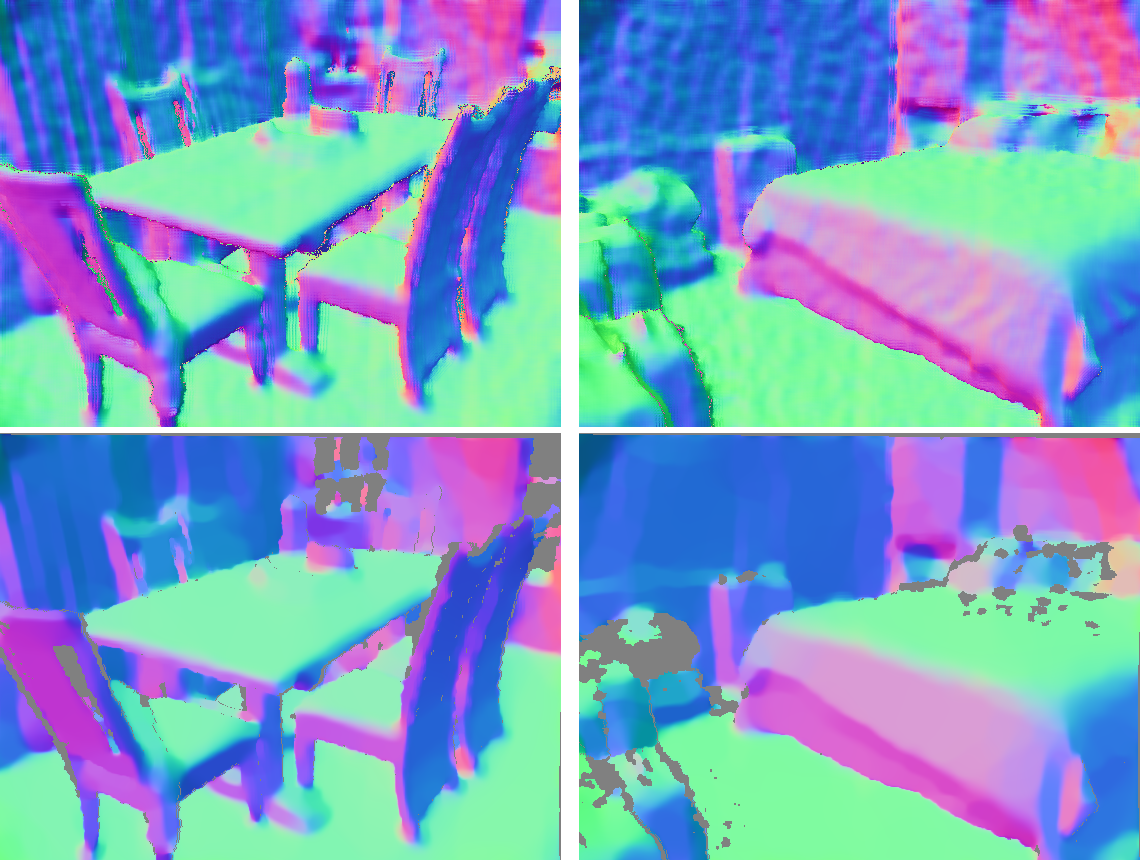
\includegraphics[width=\textwidth]{DenoisedSilberman}
    \caption{Top: normal maps computed based on the method of \citeauthor*{silberman} \cite{silberman} \\ Bottom: masked normal maps after denoising (invalid values are coloured in gray). }
    \label{fig:denoisedsilberman}
\end{figure}

\section{Implementation} \label{sec:datasets}

Three different data sets were created for use in this project: 

\begin{itemize}
    \item A main data set based on the RGB images and depth maps of the NYU Depth V.2 \cite{silberman}, and surface normal maps provided by \citeauthor*{ladicky} \cite{ladicky}.
    \item An alternative data set based on the NYU Depth V.2, and surface normal maps computed based on the method of \citeauthor*{silberman} \cite{silberman}
    \item A data set based on the RGB images and depth maps of the SUN RGB-D \cite{sun}, and surface normal maps computed based on the method of \citeauthor*{silberman} \cite{silberman}
\end{itemize}

\pagebreak

MathWorks MATLAB was used for developing the scripts and functions required for creating the data sets of this project. To build the main data set, first the RGB images and raw depth maps were extracted from NYU Depth V.2 data set. The raw depth data was used to create a mask of invalid data points in each sample (i.e. pixels with missing or invalid depth values). Then, the surface normal maps provided by \citeauthor*{ladicky} were loaded and decoded. These normal maps are provided as PNG images. Because, it was not possible to find any information about the encoding used in the process of converting the original normal maps to these images, the histograms of each channel in several samples were manually analysed to develop a decoding function. Finally, the RGB images and corresponding masked normal maps were stored in a MAT file as output.

To create the alternative data set, similar to main data set, the RGB images and the masks of invalid data points were extracted. The surface normal maps were computed and a denoising technique was applied as discussed in section \ref{sec:surfnormmap}. The masked surface normal maps and RGB images were stored in a MAT file as output.

As mentioned before, the SUN RGB-D data set consists of RGB images and refined depth images in PNG format. To explore the effect of using higher quality samples in this project, only the subset of SUN RGB-D data set is used that has corresponding images in NYU Depth V.2 data set. 

A meta-data data set and a toolbox are also provided for loading and manipulation of data. To create the last data set, the full resolution RGB and raw depth images were loaded by using the information provided in meta-data data set. Similar to the data provided by \citeauthor*{ladicky}, a custom encoding was used for storing the original data in PNG format. Surface normal maps were computed based on the raw depth data and denoising applied on the results. Finally, the RGB images and corresponding masked normal maps were stored in a MAT file.

Figure \ref{fig:sunvsnyu} illustrates the difference in quality of samples obtained from different data sets. In general, samples based on the data obtained from SUN RGB-D have less invalid values (coloured in gray) and slightly less noise. 

\begin{figure}
    \centering
    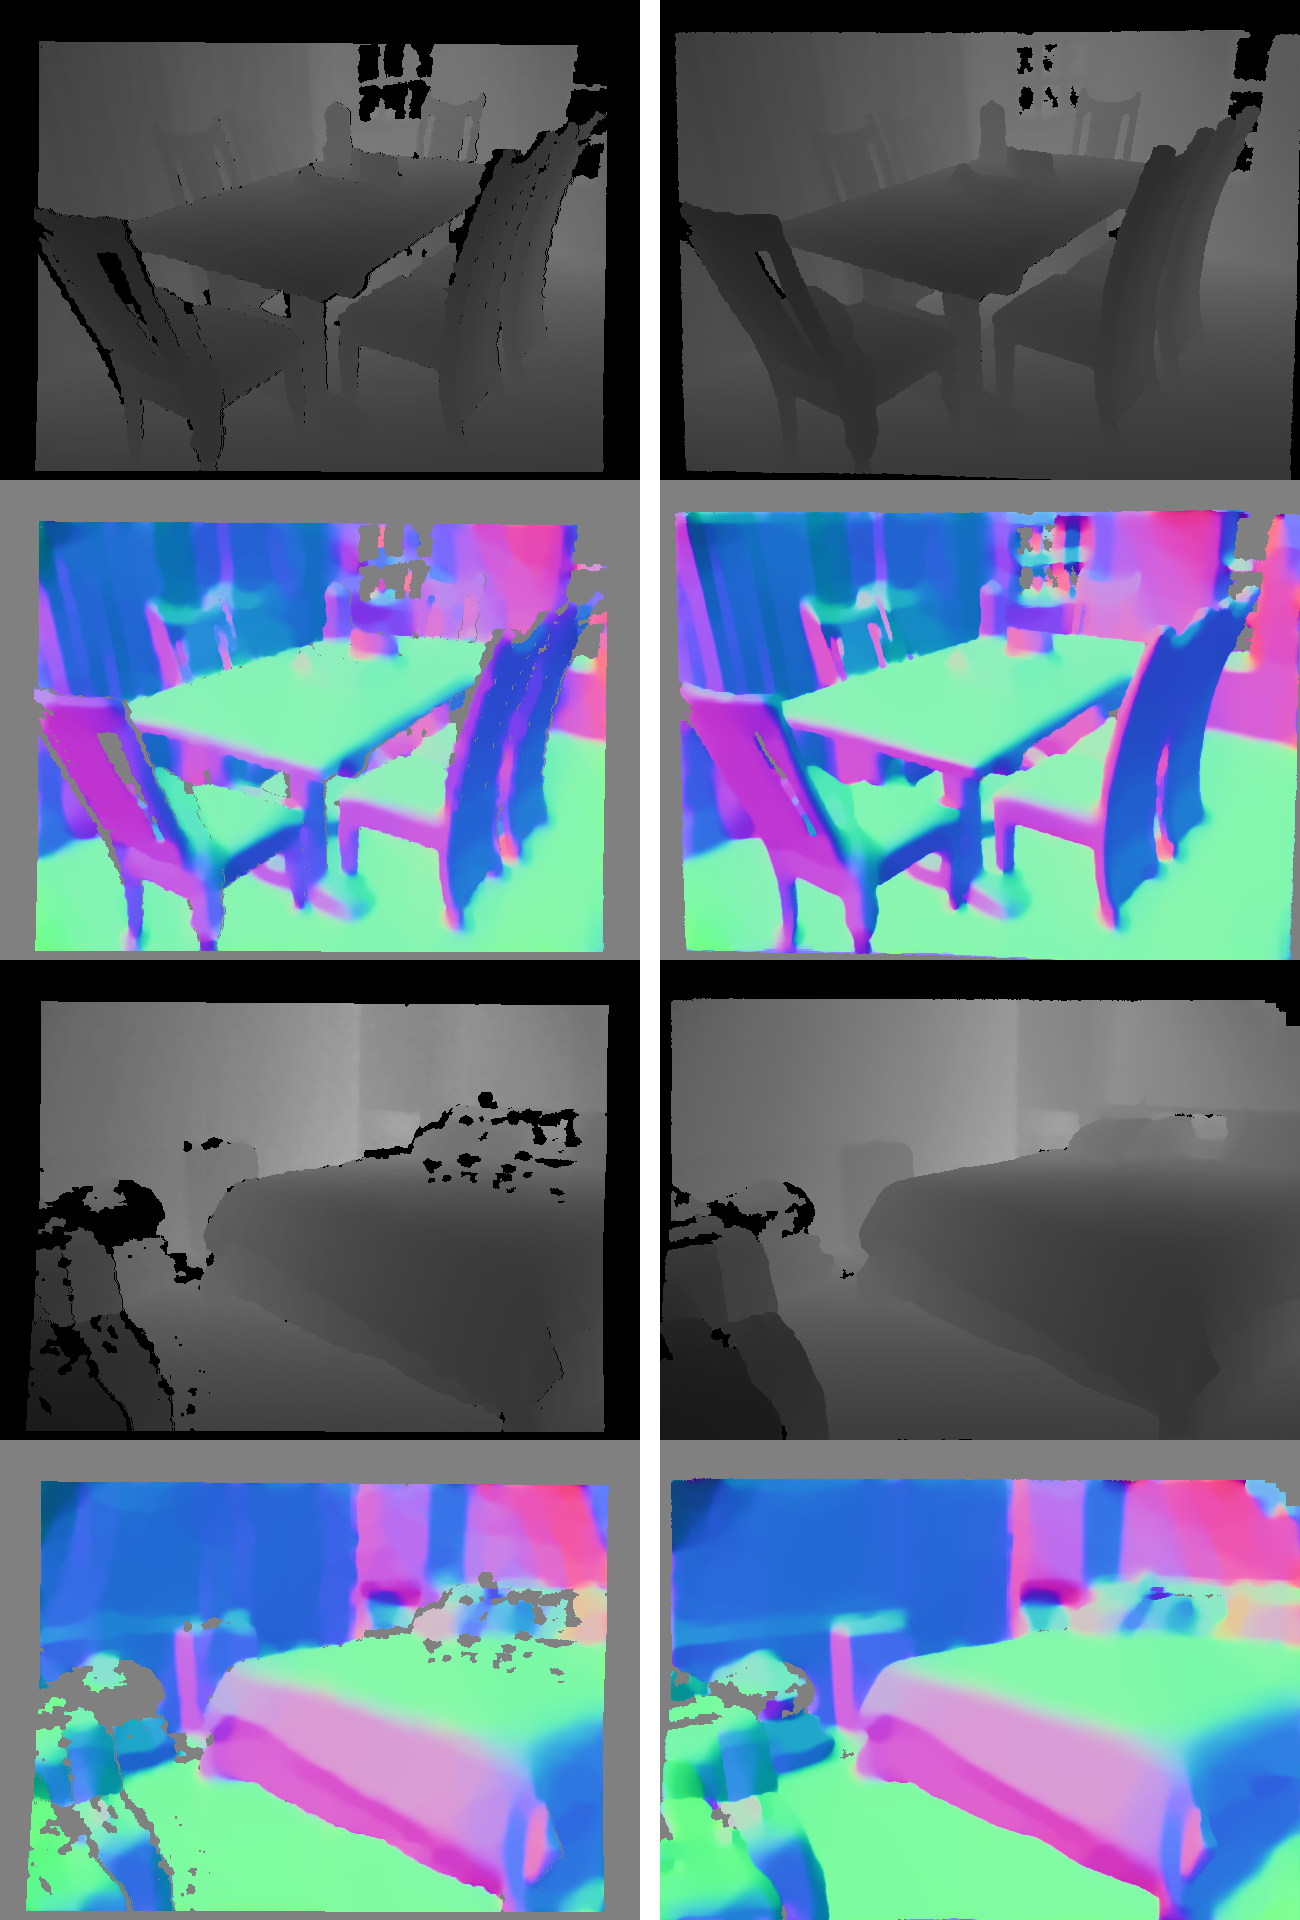
\includegraphics[width=\textwidth]{SUNvsNYU}
    \caption{Left: depth and surface normal maps based on NYU Depth V.2 \\ Right: depth and surface normal maps based on SUN RGB-D}
    \label{fig:sunvsnyu}
\end{figure}

The instructions for obtaining the data sets and source codes are provided in appendix \ref{sec:instructions}. During the development, to ensure the validity and quality of the outputs, code snippets were interactively tested and the output variables were inspected after each modification in their values.




\chapter{Model Architecture}
\label{ModelArchitecture}

\section{Baseline}
\lipsum[1-1]
\chapter{Training}
\label{Training}

\section{Overview}
\section{Data Augmentation}
\section{Experiments}


\chapter{Evaluation and Results}
\label{EvaluationAndResults}

\section{Metrics}
\section{Quantitative results}
\section{Qualitative results}
\section{Discussion}
\subsection{Achievements}
\subsection{Future Work}
\subsection{Personal Reflection}
\chapter{Conclusion}
\label{Conclusion}

\lipsum[1-1]

%Adds References to the table of content
%all you bibtex enteries go in the file called refs.bib
\addcontentsline{toc}{chapter}{References}
\bibliography{refs}

%any appendices you have go in a file called appendix.
\begin{appendices}
\chapter{External Material}
\lipsum[3-3]
\chapter{Ethical Issues Addressed}
\end{appendices}
\end{document}

